\subsection{Data Exploration}

During the first stages of the project, we implemented prototypes that helped us better understand the goal of the project
and the steps needed to achieve it.
We defined a smaller objective, which would be achieved during the first few weeks of work.
This objective was the construction of a clear map of our data.
In order to gain insights from an unstructured dataset, we first need to extract as much information about it as possible
and represent it in a structured manner.
This is called metadata.
Ralph Kimball describes metadata as ``the DNA of the data warehouse''\cite{Kimball2008} because of its importance in how data is stored.
Exploring the input by extracting and structuring metadata became the first preliminary goal of the project, which we tried
to achieve through prototypes.
\bigbreak
We split this goal further into steps:
\begin{itemize}
    \item Extract basic information about each file (size, number of rows, column names, data types, aggregate functions)
    \item Represent the extracted information in a human-readable manner
    \item Store the metadata in an efficient format
    \item Build potential relationships between files through column matching
    \item Store the results from column matching as metadata
\end{itemize}

\subsection{Column Matching Methods}

Column matching is a naive approach to data discovery.
Just because two columns look similar, it does not mean that the tables are related.
However, it is a good starting point.
Knowing if a table is timestamped and, if it is, which column holds the date \& time information, is incredibly useful for
the larger goal of the project.
In the beginning, we look at two files and try to match columns through various similarity techniques.
The results produced (as, for example, percentages) are then stored together with the rest of the metadata.
In later steps, we can use them to ``label'' columns or tables against an established set of templates.

\bigbreak

We identified three components which can tell whether two columns contain the same kind of data: the column name, the data
type and the content.
The first two are quick to analyse but provide little insight or may even point us in the wrong direction, while the third
element is reliable, but can have a big impact on performance.
Data similarity is an ambiguous topic, but we will nonetheless try to find methods of completing this task, for each of the
three elements of a column.
The results will be expressed as percentages, which we will then average into a final value representing the
\textit{degree of certainty} that two columns contain the same kind of data.

\bigbreak

If we look at column names as strings of characters, we can determine the longest continuous matching subsequence (LCS) between
the two strings, using, for example, Python's \textit{SequenceMatcher} class.
This also provides a method which produces a ratio of similarity, based on the amount of remaining characters after computing the LCS\@.
This approach seems to yield good results when the column names are similar in terms of characters.
An alternative is the Levenshtein distance, which can more accurately show the difference between two sequences.
To improve the quality of results, we can explore another facet of the column names: their meaning.
If we look at these strings as words, we can use a dictionary to check their similarity.

\subsubsection{A comparison between three methods of determining column name similarity}
Word similarity is a vast topic, and it becomes even larger when considering the possibility that column names are not
necessarily words from the dictionary.
We conducted an investigation into the difference between the three methods identified above of exploring this topic,
in order to determine which would be the most beneficial for our project, or whether we should use them together.
Initial tests were run on a hardcoded list of common column names in a commercial or managerial database: customer\_id,
first\_name, last\_name, phone, email, workdept, salary, deptnumb, manager, majproj, etc.

\bigbreak

We ran three algorithms on all pairs of terms in this list:
\begin{itemize}
    \item Longest Continuous (Matching) Subsequence (LCS), as implemented by the Python \textit{difflib} library~\cite{difflib}
    \item The Levenshtein distance, as implemented by the Python \textit{Levenshtein} library~\cite{Levenshtein}
    \item The Wu-Palmer Similarity, as implemented by the Python Natural Language Toolkit (NLTK)~\cite{wordnet}
\end{itemize}

\bigbreak

We developed two different views of the results of these tests, to compare and contrast them.
The first one is the table in fig~\ref{fig:lcs_levenshtein_wupalmer_results}.

\begin{figure}[h]
    \centering
    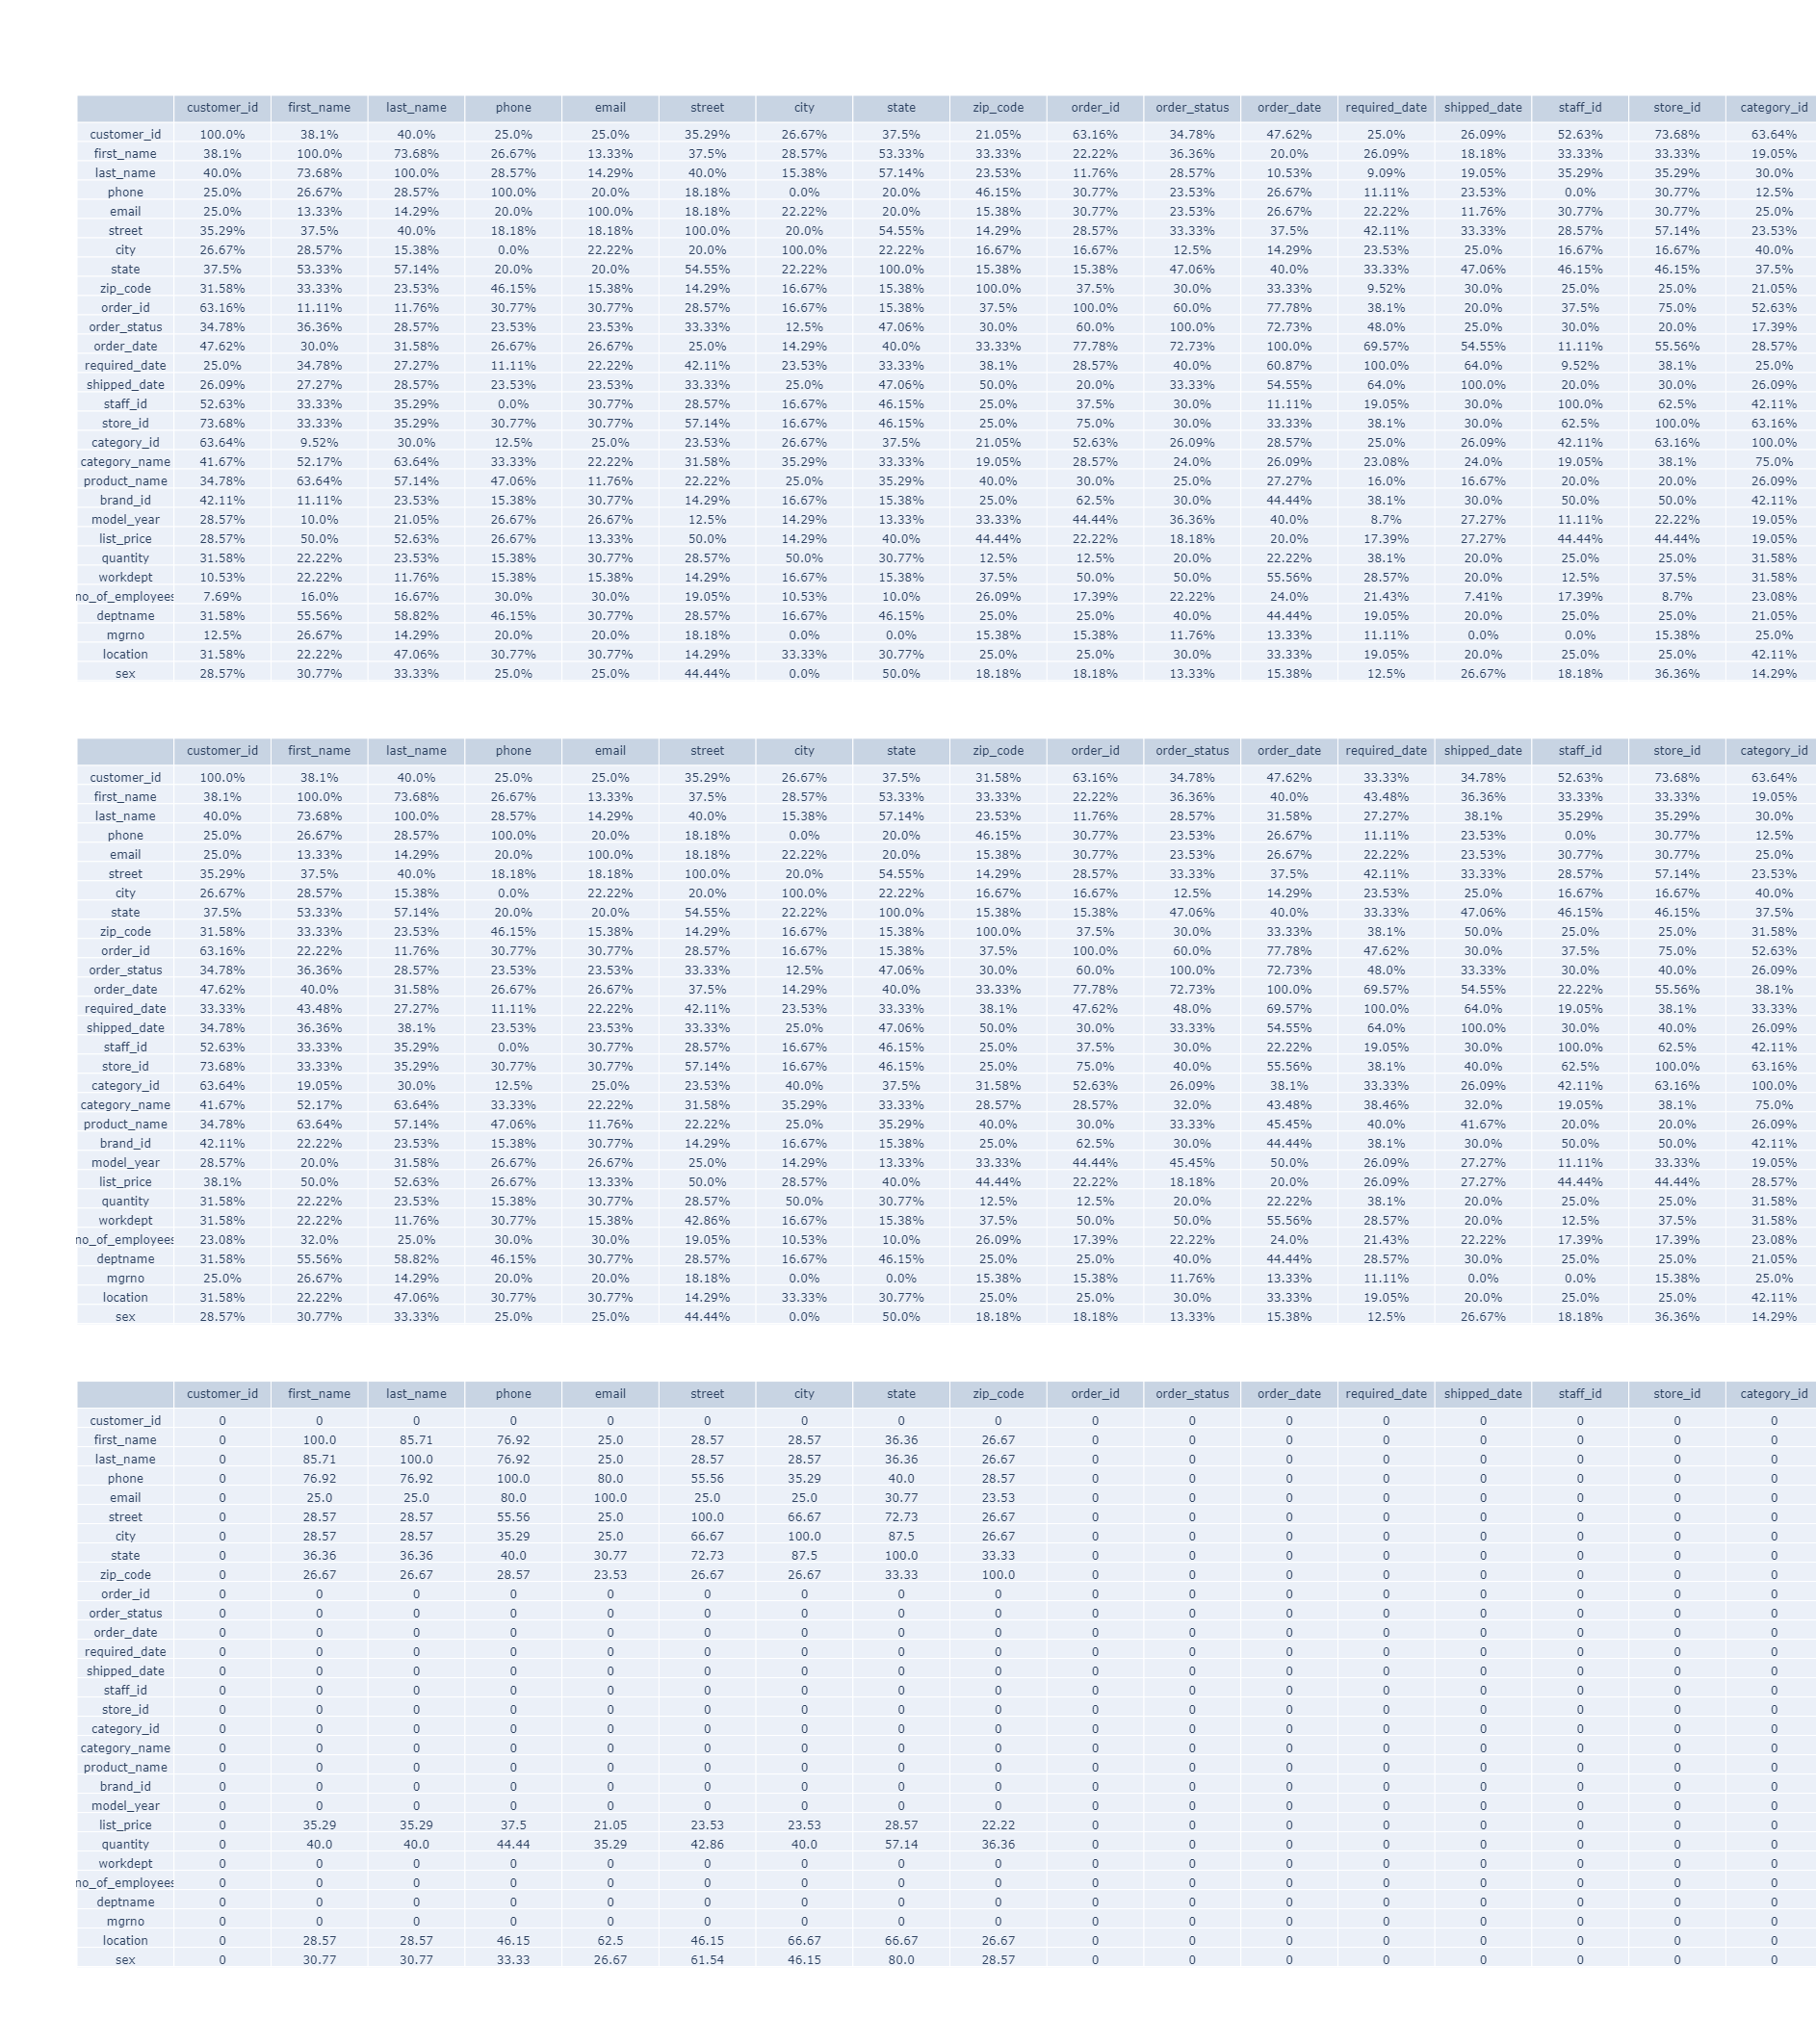
\includegraphics[width=12cm]{figures/names_lcs_levenshtein_wordnet_table}
    \caption{Full results of LCS, Levenshtein, and Wu-Palmer on a list of column names}
    \label{fig:lcs_levenshtein_wupalmer_results}
\end{figure}

Due to its size, it is difficult to extract any meaningful information from this table.
Nevertheless, at a first glance, we can observe that the values in the LCS and Levenshtein tables are almost identical,
while the Wu-Palmer table contains several zeroes.
To understand these results a bit better, we will a second display method: the best three matches, ranked by percentage,
for each column name.

\begin{verbatim}
hiredate:
	birthdate 70.59%, required_date 66.67%, store_id 37.5% [lcs]
	birthdate 70.59%, required_date 66.67%, firstname 47.06% [levenshtein]
	 0%,  0%,  0% [wordnet]

phone_no:
	phone 76.92%, projno 57.14%, order_id 37.5% [lcs]
	phone 76.92%, projno 57.14%, order_id 37.5% [levenshtein]
	 0%,  0%,  0% [wordnet]

job:
	projno 44.44%, majproj 40.0%, bonus 25.0% [lcs]
	projno 44.44%, majproj 40.0%, bonus 25.0% [levenshtein]
	position 93.33%, zip_code 63.16%, manager 63.16% [wordnet]

position:
	location 62.5%, projno 42.86%, deptname 37.5% [lcs]
	location 62.5%, projno 42.86%, store_id 37.5% [levenshtein]
	location 100.0%, job 93.33%, quantity 61.54% [wordnet]

firstname:
	first_name 94.74%, lastname 70.59%, deptname 58.82% [lcs]
	first_name 94.74%, lastname 70.59%, deptname 58.82% [levenshtein]
	 0%,  0%,  0% [wordnet]

lastname:
	last_name 94.12%, firstname 70.59%, category_name 57.14% [lcs]
	last_name 94.12%, firstname 70.59%, category_name 57.14% [levenshtein]
	 0%,  0%,  0% [wordnet]
\end{verbatim}

This is a fragment of the results displayed as the best three matches for each column name.
Every row represents the results of one method used.
Once again, we observe that LCS and Levenshtein results are very similar.
In cases where they do differ, they seem to both miss the mark.
For example, LCS matches \textit{hiredate} with \textit{store\_id} with a 37.5\% confidence, while Levenshtein matches
\textit{hiredate} with \textit{firstname} with a 47.06\% confidence.
Both pairs of column are most likely unrelated.
However, when it comes to column names with slight variations in spelling, such as \textit{lastname} and \textit{last\_name},
both LCS and Levenshtein produce correct matches with a 90\% or higher confidence.
Wu-Palmer (wordnet) fails to match columns that are not correctly spelled words in the dictionary.
On the other hand, Wu-Palmer can find matches that are essentially invisible to LCS and Levenshtein.
For example, it matches \textit{position} with \textit{location} with a 100\% confidence, which is correct (both of these
columns might contain physical locations), but it also matches \textit{position} with \textit{job} with a 93.33\% confidence,
which is also a valid option (position might refer to an employee's function in a company).

\subsubsection{Understanding the results}
According to the Python documentation, the algorithm behind SequenceMatcher predates an algorithm published by Ratcliff
and Obersheldp in the late 1980's under the hyperbolic name ``gestalt pattern matching''~\cite{difflib}.
The idea is to find the longest contiguous matching subsequence, and then apply it recursively to the sequences to the
left and right of the matching subsequence~\cite{difflib}.
The \textit{ratio()} method return a float in the range [0, 1] with the formula 2.0 * M / T, where T is the total number
of elements in both sequences and M is the number of matches~\cite{difflib}.
The Levenshtein distance between two strings is the number of insertions, deletions, or substitutions required to transform
one string into the other.
A C extension module for Python implements the ratio of similarity between two strings as the complement of the normalized
Levenshtein distance~\cite{Levenshtein}.
Given these implementations of LCS and Levenshtein, it makes sense that the results obtained are very similar.
Both methods look at how close two strings are character by character.
Therefore, the best usage of these methods in column name matching is to combine them.
Disagreements with a low confidence percentage can be ignored, but disagreements with a high confidence should be resolved
by applying a different comparison method, such as Wu-Palmer.

\bigbreak

WordNet is an interface for Python's NLTK module.
According to its documentation, WordNet structures words using synsets, which are, essentially, sets of synonyms that
share a common meaning~\cite{wordnet}.
Each synset contains one or more lemmas, which represent a specific sense of a specific word~\cite{wordnet}.
The Wu-Palmer similarity is implemented as ``a score denoting how similar two word senses are, based on the depth of the
two senses in the taxonomy and that of their Least Common Subsumer (most specific ancestor node)''~\cite{wordnet}.
This explains why our Wu-Palmer test was able to match \textit{position} and \textit{location}, but also \textit{position}
and \textit{job}, both with a very high confidence.
The word ``position'' shares a synset with both ``location'' and ``job'', the first one meaning ``a place in the physical world'',
and the second one ``a function in an organization''.
This algorithm is, therefore, extremely useful for identifying columns with similar data, whose names are synonyms in the
dictionary.
The shortcomings of WordNet are visible when the words are spelled incorrectly.
For example, the algorithm might correctly identify the words \textit{first} and \textit{name}, but not \textit{firstname},
nor \textit{first\_name}, the last two being common occurrences in datasets.
A possible solution is the use of tokenization (splitting a string into words).
However, attempts to use this approach did not show an improvement of results.
That is because many of the common column names selected in the test (such as \textit{firstname} and \textit{majproj}) cannot
be tokenized.
Additionally, WordNet does not work well with phrases.
Its synsets are built with singular words, therefore it cannot grasp the meaning obtained when combining words such as
\textit{phone} and \textit{number}.

\subsubsection{Data types}
The data types provide the least amount of information about the similarity of the two columns.
We can check whether they share the same data type (numerical, strings, boolean), but this does not mean the contents
are related.
However, finding numerical data gives a strong probability that the data in the column is continuous, while finding any other
data type may show that the data is categorical.
Unfortunately, this can only be verified by looking at the data itself.
Looping through the rows and comparing them is costly.
If we are dealing with categorical data, there might be value in comparing the sets of categories and their frequencies.
Continuous, numerical data can be compared using mathematical formulas, such as the Pearson correlation coefficient.
Whichever strategy we choose, we should ensure it is as time-efficient as possible.

\bigbreak

First, we compare the data types of the two columns.
This operation is fast, as we are only using the information provided by Pandas about the dataframe~\cite{pandasDtypes}.
Furthermore, if we include the data types of the columns in the metadata, we will not need access to the dataframe at
all for this step.

The next few data analysis methods will dive into the content of the dataframes, thus increasing the time and space
complexity of executing them.
However, looking only at data types is not enough.
Data types given by Pandas can be misleading.
For example, a column of string may actually hide numbers that have been erroneously processed as strings.
Pandas provides a useful method for determining which strings in a series can be parsed as numbers, namely
\textit{to\_numeric}~\cite{pandasToNumeric}.

The \textit{coerce} parameter will set all non-numeric values to NaN, and the \textit{dropna()} method will remove them.
This function can also be used to determine the percentage of numerical values in a series and roughly equal
percentages of numerical values in two different columns can be an indicator of similarity.
We also want to determine what percentage of the entries in a series are unique.
We call this the \textit{continuity} factor and can calculate it with a simple formula: the number of unique values in the
column divide by the total number of rows.

Columns that produce a low value (below 0.5) here can be treated as categorical and two categorical columns can be
compared by looking at the unique values in each.
In particular, we want to compare the sizes of the intersection of the two series and their union.
We use NumPy's implementation of these two sets: \textit{intersect1d}~\cite{numpyIntersect1d} and
\textit{union1d}~\cite{numpyUnion1d}.
It is a good idea to transform all values in the columns into strings before performing the test, to avoid any type errors.
Then, the similarity value will be the length of the intersection divided by the length of the union.

On the other hand, numerical columns with a high continuity factor can be compared using the Pearson correlation
coefficient.
Pearson's correlation is a measurement of the linear correlation between two variables.
It takes values between -1 and 1.
A value of 1 means that for every positive increase in one variable, there is a positive increase of a fixed proportion
in the other.
A value of -1 means that positive increases in one variable are proportional to decreases
in the other~\cite{PearsonCorrelationCoefficient}.
A Pearson coefficient close to 1 would indicate a strong relation between two columns and can be used in our column
matching algorithm.
A value close to -1 can also be statistically significant, while a value around 0 would indicate no correlation.
For example, applying the Pearson coefficient to the heights and ages to the students of a school would probably indicate
a strong correlation.
One shortcoming of the correlation coefficient is that it cannot tell the difference between dependent and
independent variables~\cite{PearsonCorrelationCoefficient}.
Therefore, it would be unable to determine which is the cause and which is the effect, but it is still able to detect the
correlation in such a situation, which is what we are interested in.
Pandas has a convenient \textit{corr()} method for computing the Pearson correlation coefficient between two series or
dataframes~\cite{pandasCorr}.

The two-sample t-test is another method of comparing two numerical, continuous columns.
The two-sample t-test is used to determine whether the unknown population means of two groups are equal or not~\cite{twoSampleTTest}.
When performing this test, we propose the null hypothesis that the unknown population means of the two series are equal.
This should give a good indication of strong similarity or correlation between them.
If the resulting p-value is smaller than 5\% (a common threshold value), we can safely reject the null hypothesis and claim
that the means are different.
There are a number of preconditions that the data needs to meet in order for the two-sample t-test to be valid (the sample
sets must be independent, obtained randomly, and continuous~\cite{twoSampleTTest}), therefore we should use this method
carefully in our data matcher.
The calculations involved in the test also differ when the two sample sets have equal variances or not.
For the Python implementation, we will use the method \textit{ttest\_ind()} in the \textit{scipy} library~\cite{scipyTwoSampleTTestInd}.
We must first determine the equality of the variances of the two series and pass it to \textit{ttest\_ind()} as a parameter.
Then, running this method will give us the p-value we require.

\subsubsection{Stationarity}
A stationary process is ``a stochastic process whose unconditional joint probability distribution does not change when shifted
in time''~\cite{Gagniuc2017}.
In other words, it is ``a flat looking series, without trend, constant variance over time, a constant autocorrelation structure
over time and no periodic fluctuations''~\cite{EngineeringStatisticsHandbook}.
Determining whether our continuous data is stationary or not could be the first step towards trend analysis and prediction.
Stationarity can by itself be an indication of similarity (for example, temperature measurements taken at the same place
in the same season should be stationary), but it should be combined with other kinds of analysis for higher accuracy.
One method of determining stationarity is the Augmented Dickey-Fuller Test (ADF).
ADF tests the null hypothesis that a unit root is present in a time-series sample~\cite{Greene1997}.
If a unit root is present in a stochastic process, then that process is non-stationary, but it does not necessarily have a trend.
Therefore, the alternate hypothesis of the ADF test is that the series is stationary.
ADF uses the p-value to accept or reject the null hypothesis, but it also produces a secondary value, called the ADF statistic.
The more negative this number is, the stronger the confidence in rejecting the null hypothesis~\cite{Greene1997}.

\bigbreak

The Python library \textit{statsmodels} contains an implementation of ADF~\cite{statsmodels}, which we applied to data produced
by our generator.
Our test dataframes are composed of two columns and one hundred rows.
The first column is an index, and will always have values from 0 to 99.
Running ADF on this series produces an ADF statistic of approximately 2.46 and a p-value of 0.99.
This is extremely strong evidence for accepting the null hypothesis that this series is non-stationary, which must be true
for a linear, incremental process.
The second column will always contain continuous data following a sine wave.
All tests on this column produced small ADF statistic values, around -5000000000000.
The p-value was shown as 0.0, indicating that it was a positive number very close to 0.
This evidence points towards confidently rejecting the null-hypothesis that the series has a root value and claiming that
a sine wave is stationary, which, once again, is true.

\bigbreak

\subsubsection{Dynamic Time Warping}
Determining stationarity for a data series is useful, but, going further, we would also like to know if two series follow
the same pattern or trend.
For example, if two datasets measure the same parameter over a time period (say, temperature), but use different units of
measurement, they will show the same trend, and we would like to catalogue them under the same category, or even merge them.
One way to achieve this is dynamic time warping (DTW).
In the paper ``Dynamic Time Warping Algorithm Review'', Pavel Senin explains that the algorithm builds a distance matrix
between all points in the first series and all points in the second series.
Then, the algorithm finds the ``alignment path which runs through the low-cost areas of the cost matrix''~\cite{DTWAlgorithmReview},
and associates a cost function to it.
The path with the lowest cost associated with alignment will be the optimal path~\cite{DTWAlgorithmReview}.
The alignment path must satisfy a number of conditions, which, in short, ensure that warping the first time series to the second one
preserved the chronological ordering of the points.
The result of this algorithm is the minimal cost incurred by transforming one series to make it identical to the other.
The smaller this cost, the higher the similarity of the two series.
To calculate this similarity percentage, we compute an auxiliary value MAX\_DIST, equal to the length of the first series
times its maximum value, guaranteed to be larger than the biggest obtainable distance.
Then, the similarity percentage will be (MAX\_DIST - distance) / MAX\_DIST * 100.
We want to keep MAX\_DIST close to the real distance values, because using an abnormally high boundary wil produce percentages
that accumulate towards 100\% and will make interpreting the results more difficult.
One limitation of DTW is that the data points in both series must be sampled at equidistant points in time.
Another one is its time complexity.
DTW runs in O(N*M), where N and M are the sizes of the two series.
Therefore, if we are dealing with large data sets, we can only apply DTW on small chunks of them.

\bigbreak

We ran the DTW algorithm on some data sets produced by our generator, with two kinds of continuous data: indexes (linear and
incremental) and sine waves.
Comparing two distinct sine waves yielded similarity scores of 95\% and above, while comparing an index with a sine wave produced
an average similarity of 50\%.
This gives a clear indication of whether two data series should be considered similar or not and will help us set a confidence
threshold when applying DTW in combination with other methods.
Additionally, we observed that the algorithm's runtime increases significantly (from a few seconds to a few minutes) when
changing the size of the data series from 1000 points to 10000.
